\documentclass[../cours_3e.tex]{subfiles}
\begin{document}
\setcounter{chapter}{12}
\chapter{Le théorème de Pythagore}
\label{ch:pythagore}
\begin{objectif}
Calculer une longueur dans un triangle rectangle, reconnaître un angle droit et distinguer théorème, réciproque et contraposée. Prérequis : aires, carrés et racines.
\end{objectif}
\section{Énoncé et vocabulaire}
\begin{definition}
Dans un triangle rectangle, l'hypoténuse est le côté opposé à l'angle droit. C'est le plus long côté.
\end{definition}
\begin{theoreme}[Pythagore]
Si le triangle $ABC$ est rectangle en $A$, alors
\[BC^2=AB^2+AC^2.\]
Le carré de l'hypoténuse est la somme des carrés des deux autres côtés.
\end{theoreme}
\begin{center}
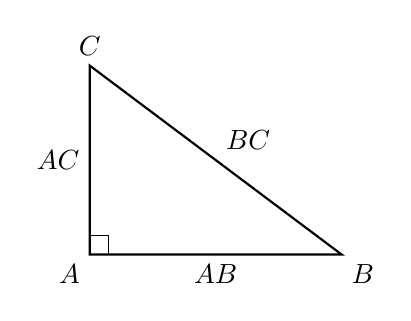
\begin{tikzpicture}[scale=.8]
\coordinate(A)at(0,0);\coordinate(B)at(4,0);\coordinate(C)at(0,3);
\draw[thick](A)--node[below]{$AB$}(B)--node[above right]{$BC$}(C)--node[left]{$AC$}cycle;
\draw(.3,0)--(.3,.3)--(0,.3);
\node[below left]at(A){$A$};\node[below right]at(B){$B$};\node[above]at(C){$C$};
\end{tikzpicture}
\end{center}
Le théorème implique que l'hypoténuse est la plus longue : $BC^2>AB^2$ et $BC^2>AC^2$, puisque les côtés sont strictement positifs.
\section{Une démonstration par les aires}
Prenons un triangle rectangle dont les côtés de l'angle droit mesurent $a,b$ et l'hypoténuse $c$. Plaçons quatre copies dans un carré de côté $a+b$.
\begin{center}
\begin{tikzpicture}[scale=.9]
\draw[thick](0,0)rectangle(5,5);
\filldraw[fill=accent!18,draw=accent,thick](3,0)--(5,3)--(2,5)--(0,2)--cycle;
\node at(2.5,2.5){aire $c^2$};
\node[below]at(1.5,0){$a$};\node[below]at(4,0){$b$};
\node[right]at(5,1.5){$a$};\node[right]at(5,4){$b$};
\node[above]at(3.5,5){$a$};\node[above]at(1,5){$b$};
\node[left]at(0,3.5){$a$};\node[left]at(0,1){$b$};
\node[rotate=56.3]at(4.05,1.35){$c$};
\end{tikzpicture}
\end{center}
\begin{demonstration}
Le quadrilatère central a quatre côtés de longueur $c$. Chaque angle central est droit, car les deux angles aigus d'un triangle rectangle ont pour somme $90\degre$ ; avec eux, l'angle central forme un angle plat. Le centre est donc un carré.

L'aire du grand carré vaut $(a+b)^2$. Elle est aussi la somme du carré central et des quatre triangles :
\[(a+b)^2=c^2+4\frac{ab}{2}=c^2+2ab.\]
Or $(a+b)^2=a^2+2ab+b^2$. En retirant $2ab$, on obtient $a^2+b^2=c^2$.
\end{demonstration}
La figure n'est pas seulement une illustration : elle indique un découpage dont les propriétés et les aires ont été justifiées.
\section{Calculer une longueur}
\begin{methode}
Identifier le triangle rectangle et son angle droit. Écrire l'égalité avec les lettres. Remplacer par les longueurs connues. Isoler le carré cherché. Prendre la racine positive et donner une valeur exacte puis l'arrondi demandé.
\end{methode}
\begin{exemple}[Chercher l'hypoténuse]
Dans $ABC$ rectangle en $A$, $AB=6\unite{cm}$ et $AC=8\unite{cm}$ :
\[BC^2=6^2+8^2=100,\qquad BC=\sqrt{100}=10\unite{cm}.\]
\end{exemple}
\begin{exemple}[Chercher un côté de l'angle droit]
Si l'hypoténuse mesure $13\unite{cm}$ et un autre côté $5\unite{cm}$, le troisième côté $x$ vérifie
\[13^2=5^2+x^2,\qquad x^2=169-25=144,\qquad x=12\unite{cm}.\]
\end{exemple}
\begin{exemple}[Valeur non entière]
Pour un rectangle de côtés $4$ et $7\unite{cm}$, la diagonale vaut $\sqrt{4^2+7^2}=\sqrt{65}\unite{cm}\approx8{,}06\unite{cm}$. Arrondie au millimètre, elle vaut $8{,}1\unite{cm}$.
\end{exemple}
\begin{attention}
Les longueurs doivent avoir la même unité. On n'écrit pas $c=a+b$ : c'est l'égalité des \emph{carrés} qui est vraie. Si le triangle n'est pas connu rectangle, Pythagore ne peut pas être utilisé directement.
\end{attention}
\section{Réciproque : prouver qu'un triangle est rectangle}
\begin{theoreme}
Dans un triangle $ABC$, si $BC^2=AB^2+AC^2$, alors le triangle est rectangle en $A$.
\end{theoreme}
\begin{demonstration}
Construire un triangle $A'B'C'$ rectangle en $A'$ avec $A'B'=AB$ et $A'C'=AC$. Le théorème direct donne $B'C'^2=AB^2+AC^2=BC^2$, donc $B'C'=BC$ car les longueurs sont positives. Les deux triangles ont leurs trois côtés égaux : par CCC, ils sont superposables. L'angle en $A$ est donc droit.
\end{demonstration}
\begin{exemple}
Un triangle a pour côtés $7{,}5$, $10$ et $12{,}5\unite{cm}$. Le plus long côté est $12{,}5$. On calcule séparément :
\[12{,}5^2=156{,}25,\qquad7{,}5^2+10^2=56{,}25+100=156{,}25.\]
Les valeurs sont égales : le triangle est rectangle en face du côté de $12{,}5\unite{cm}$.
\end{exemple}
\section{Contraposée : prouver qu'il ne l'est pas}
Si le carré du plus long côté n'est pas égal à la somme des deux autres carrés, le triangle n'est pas rectangle. Sinon le théorème direct imposerait justement cette égalité.
\begin{exemple}
Pour des côtés $4$, $6$ et $7$, on a $7^2=49$ tandis que $4^2+6^2=52$. Le triangle n'est pas rectangle.
\end{exemple}
\begin{attention}
Des valeurs arrondies ne suffisent pas toujours à conclure sur un angle exactement droit. La réciproque exige l'égalité exacte des longueurs données, pas une simple proximité due à la mesure.
\end{attention}
\section{Applications : distance et espace}
Dans un repère \textbf{orthonormé}, le triangle formé par les déplacements horizontal et vertical entre $A(x_A;y_A)$ et $B(x_B;y_B)$ est rectangle :
\[AB=\sqrt{(x_B-x_A)^2+(y_B-y_A)^2}.\]
C'est une application de Pythagore ; la formule n'est pas à appliquer telle quelle si les unités graphiques des axes diffèrent.
Dans un pavé droit de dimensions $a,b,c$, appliquer deux fois Pythagore donne une grande diagonale de longueur $\sqrt{a^2+b^2+c^2}$ : d'abord $\sqrt{a^2+b^2}$ dans la base, puis avec la hauteur $c$.
\utilite{Calculer une diagonale, une hauteur inaccessible ou un trajet direct ; vérifier un équerrage ; trouver le rayon d'une section de sphère.}
\begin{retenir}
Angle droit connu : théorème direct. Longueurs connues et égalité exacte : réciproque. Égalité non vérifiée : contraposée. Toujours commencer par identifier le plus long côté.
\end{retenir}
\end{document}
